\documentclass{article}
\usepackage[shortlabels]{enumitem}
\usepackage{amsmath, amssymb, graphicx, mathtools, nicefrac, verbatim}
\usepackage[letterpaper, margin = 1in]{geometry}
\usepackage{makecell}
\usepackage{adjustbox}
\graphicspath{{imgs/}}
\newcommand{\specialcell}[2][c]{%
  \begin{tabular}[#1]{@{}c@{}}#2\end{tabular}}
\usepackage{cprotect}
\title{Group 18: CSCE 312 CPU Project | Final Report}
\author{Lucian Chauvin \\ 133003371 \\\And Joshua Lass \\ 531009387 \\\And Bjorn Quarfordt \\ 230003985}
\begin{document}
\maketitle
    \vspace{-1cm}
\section{Transformation Tables}
\begin{center}
\begin{adjustbox}{width=\columnwidth,center}
\begin{tabular}{|l|l|l|l|l|l|l|}
    \hline 
    Instruction & Fetch & Decode & Execute & Memory & Write Back & PC Update	 \\
    \hline 
    \verb+rrmovq rA, rB+ & \begin{tabular}[x]{@{}l@{}}\verb+icode:ifun+$\leftarrow $ \verb+M_1[PC]+\\\verb+rA:rB+ $\leftarrow$ \verb!M_1[PC+1]!\\ \verb+valP+$\leftarrow $ \verb!PC+2!\end{tabular} & \begin{tabular}[x]{@{}l@{}}\verb+valA+$ \leftarrow$ \verb+R[rA]+\\\verb+valB+$\leftarrow$ \verb+R[rB]+ \end{tabular} &  &  & \verb+R[rB]+$\leftarrow $ \verb+valA+ & \verb+PC+$\leftarrow $ \verb+valP+ \\
    \hline
    \verb+irmovq V, rB+ & \begin{tabular}[x]{@{}l@{}}\verb+icode:ifun+ $\leftarrow $ \verb+M_1[PC]+ \\ \verb+F:rB+ $\leftarrow $ \verb!M_1[PC+1]! \\ \verb+valC+ $\leftarrow $ \verb!M_8[PC+2]! \\ \verb+PC+ $\leftarrow $ \verb!PC+10!\end{tabular} &  &  &  & \verb+R[rB]+ $\leftarrow $ \verb+valC+ & \verb+PC+ $\leftarrow $  \verb+valP+	 \\
    \hline
    \verb+rmmovq rA, D(rB)+ & \begin{tabular}[x]{@{}l@{}}\verb+icode:ifun+ $\leftarrow$  \verb+M_1[PC]+\\\verb+rA:rB+ $\leftarrow$ \verb!M_1[PC+1]! \\ \verb+valC+ $\leftarrow$ \verb!M_8[PC+2]! \\ \verb!valP! $\leftarrow$ \verb!PC+10! \end{tabular}& \begin{tabular}[x]{@{}l@{}}\verb+valA+$ \leftarrow$ \verb+R[rA]+\\\verb+valB+$\leftarrow$ \verb+R[rB]+\end{tabular} & \verb+valE+$\leftarrow$\verb!valB+valC! & \verb+M_8[valE]+$\leftarrow $ \verb+valA+ &  & \verb+PC+ $\leftarrow $ \verb+valP+	 \\
    \hline
    \verb+mrmovq D(rB), rA+ & \begin{tabular}[x]{@{}l@{}}\verb+icode:ifun+ $\leftarrow$  \verb+M_1[PC]+\\\verb+rA:rB+ $\leftarrow$ \verb!M_1[PC+1]! \\ \verb+valC+ $\leftarrow$ \verb!M_8[PC+2]! \\ \verb!valP! $\leftarrow$ \verb!PC+10! \end{tabular}& \begin{tabular}[x]{@{}l@{}}\verb+valB+$\leftarrow$ \verb+R[rB]+\end{tabular} & \verb+valE+$\leftarrow$\verb!valB+valC! &\verb+valM+ $\leftarrow $ \verb+M_8[valE]+ & \verb+R[rA]+$\leftarrow $ \verb+valM+ & \verb+PC+ $\leftarrow $ \verb+valP+	 \\
    \hline
        \verb+OPq rA, rB+ & \begin{tabular}[x]{@{}l@{}}\verb+icode:ifun+$\leftarrow $ \verb+M_1[PC]+\\\verb+rA:rB+ $\leftarrow$ \verb!M_1[PC+1]!\\ \verb+valP+$\leftarrow $ \verb!PC+2!\end{tabular} & \begin{tabular}[x]{@{}l@{}}\verb+valA+$ \leftarrow$ \verb+R[rA]+\\\verb+valB+$\leftarrow$ \verb+R[rB]+ \end{tabular} & \verb+valE+$\leftarrow $ \verb+valB OP valA+ &  & \verb+R[rB]+$\leftarrow $ \verb+valE+ & \verb+PC+$\leftarrow $ \verb+valP+	 \\
        \hline
    \verb+jXX Dest+ & \begin{tabular}[x]{@{}l@{}}\verb+icode:ifun+$\leftarrow $ \verb+M_1[PC]+\\\verb+valC+ $\leftarrow$ \verb!M_1[PC+1]!\\ \verb+valP+$\leftarrow $ \verb!PC+9!\end{tabular}  &  & \begin{tabular}[x]{@{}l@{}}\verb+cnd+$\leftarrow $ \verb+cond(CC_1:ifun)+ \end{tabular} &  &  & \begin{tabular}[x]{@{}l@{}}\verb+PC+$\leftarrow $ \verb+cond ? valC:valP+\end{tabular} \\
    \hline
    \verb+cmovXX rA, rB+ & \begin{tabular}[x]{@{}l@{}}\verb+icode:ifun+$\leftarrow $ \verb+M_1[PC]+\\\verb+valC+ $\leftarrow$ \verb!M_1[PC+1]!\\ \verb+valP+$\leftarrow $ \verb!PC+2!\end{tabular}  & \begin{tabular}[x]{@{}l@{}}\verb+valA+$\leftarrow $ \verb+R[rA]+\end{tabular} & \begin{tabular}[x]{@{}l@{}}\verb+valE+$\leftarrow $ \verb+valA+\end{tabular}  &  & \begin{tabular}[x]{@{}l@{}}\verb+r[rB]+$\leftarrow $ \verb+valE+\end{tabular}  & \begin{tabular}[x]{@{}l@{}}\verb+PC+$\leftarrow $ \verb+valP+\end{tabular}  \\
    \hline
    \verb+call Dest+ & \begin{tabular}[x]{@{}l@{}}\verb+icode:ifun+$\leftarrow $ \verb+M_1[PC]+\\\verb+valC+ $\leftarrow$ \verb!M_8[PC+1]!\\\verb+valP+$\leftarrow $ \verb!PC+9!\end{tabular} & \begin{tabular}[x]{@{}l@{}}\verb+valB+$\leftarrow$ \verb!R[\%rsp]! \end{tabular} & \begin{tabular}[x]{@{}l@{}}\verb+valE+$\leftarrow $ \verb+valB-8+\end{tabular} & \begin{tabular}[x]{@{}l@{}}\verb+M_8[valE]+$\leftarrow $ \verb+valP+\end{tabular} & \begin{tabular}[x]{@{}l@{}}\verb+R[\%rsp]+$\leftarrow $ \verb+valE+\end{tabular} & 	\begin{tabular}[x]{@{}l@{}}\verb+PC+$\leftarrow $ \verb+valC+ \end{tabular} \\
    \hline
    \verb+ret+ & \begin{tabular}[x]{@{}l@{}}\verb+icode:ifun+$\leftarrow $ \verb+M_1[PC]+ \end{tabular} & \begin{tabular}[x]{@{}l@{}}\verb+valA+$\leftarrow $ \verb+R[\%rsp]+\\\verb+valB+$\leftarrow $ \verb+R[\%rsp]+\end{tabular}& \begin{tabular}[x]{@{}l@{}}\verb+valE+$\leftarrow $ \verb+valB_8+\end{tabular} & \begin{tabular}[x]{@{}l@{}}\verb+valM+$\leftarrow $ \verb+M_8[valA]+\end{tabular} & \begin{tabular}[x]{@{}l@{}}\verb+R[\%rsp]+$\leftarrow $ \verb+valE+\end{tabular} & \begin{tabular}[x]{@{}l@{}}\verb+PC+$\leftarrow $ \verb+valM+\end{tabular}	 \\
    \hline
    \verb+pushq rA+ & \begin{tabular}[x]{@{}l@{}}\verb+icode:ifun+$\leftarrow $ \verb+M_1[PC]+\\\verb+rA:rB+$\leftarrow $ \verb!M_1[PC+1]!\\\verb+valP+$\leftarrow $ \verb!M_8[PC+10]!\end{tabular} & \begin{tabular}[x]{@{}l@{}}\verb+valA+$\leftarrow $ \verb+R[rA]+\\\verb+valB+$\leftarrow $ \verb!R[\%rsp]!\end{tabular} & \begin{tabular}[x]{@{}l@{}}\verb+valE+$\leftarrow $ \verb+valB-8+\end{tabular} & \begin{tabular}[x]{@{}l@{}}\verb+M_8[valE]+$\leftarrow $ \verb+valA+\end{tabular} & \begin{tabular}[x]{@{}l@{}}\verb+R[\%rsp]+$\leftarrow $ \verb+valE+\end{tabular} & \begin{tabular}[x]{@{}l@{}}\verb+PC+$\leftarrow $ \verb+valP+\end{tabular}	 \\
    \hline
    \verb+pop rA+ & \begin{tabular}[x]{@{}l@{}}\verb+icode:ifun+$\leftarrow $ \verb+M_1[PC]+\\\verb+rA:rB+$\leftarrow $ \verb!M_1[PC+1]!\\\verb+valP+$\leftarrow $ \verb!M_8[PC+2]!\end{tabular} & \begin{tabular}[x]{@{}l@{}}\verb+valA+$\leftarrow $ \verb+R[\%rsp}+\\\verb+valB+$\leftarrow $ \verb!R[\%rsp]!\end{tabular} & \begin{tabular}[x]{@{}l@{}}\verb+valE+$\leftarrow $ \verb!valB+8!\end{tabular} & \begin{tabular}[x]{@{}l@{}}\verb+valM+$\leftarrow $ \verb+M_8[valA]+\end{tabular} & \begin{tabular}[x]{@{}l@{}}\verb+R[\%rA]+$\leftarrow $ \verb+valM+\\\verb+R[\%rsp]+$\leftarrow $ \verb!valE!\end{tabular} & \begin{tabular}[x]{@{}l@{}}\verb+PC+$\leftarrow $ \verb+valP+\end{tabular}	 \\
    \hline
\end{tabular}
\end{adjustbox}
\end{center}
\section{Fetch Implementation}
Our design is basically a one-to-one implementation of what is shown on the slides. Our instruction memory module stores the program in ROM and reads $10$ bytes in from the current \verb+PC+. We then pass these $10$ bytes to our align module which | based on if we need registers or not | sets out \verb+rA+, \verb+rB+, and \verb+valC+ correctly. We determine whether we need registers based on the value of \verb+icode+. Then based on if we read in registers or if we read in a  \verb+valC+ we increment our \verb+PC+ using our PC increment module.
\subsection{Fetch}
\begin{center}
    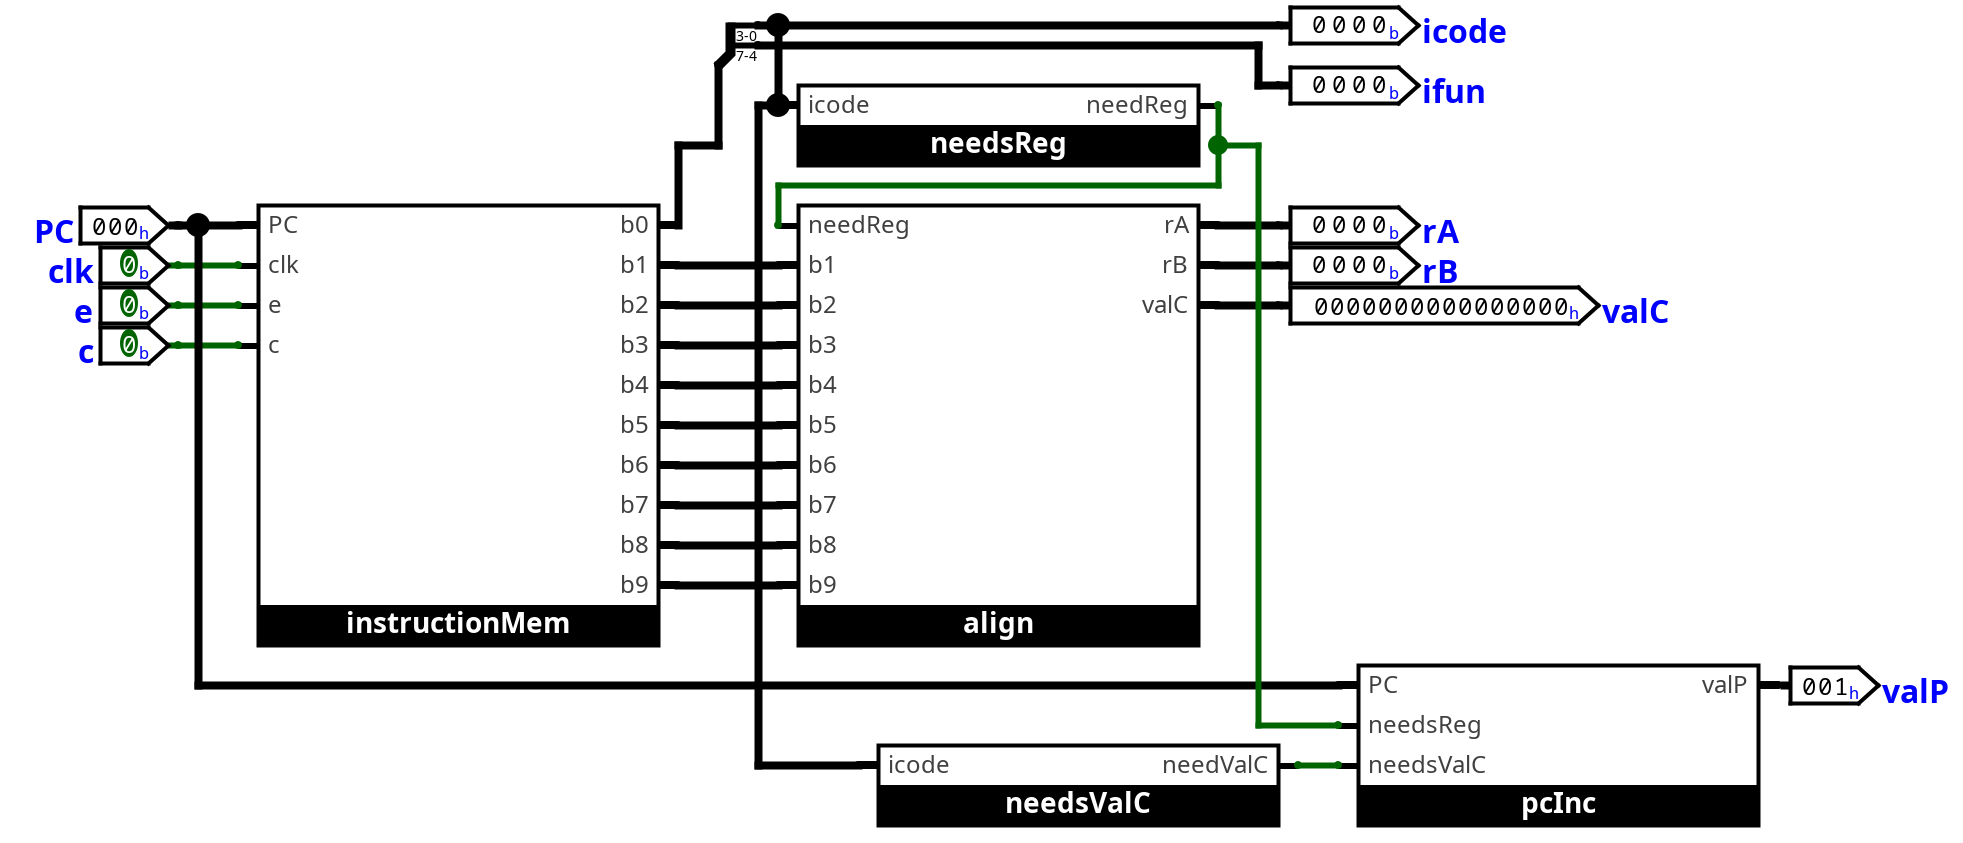
\includegraphics[scale=.7]{fetch.png}
\end{center}
\subsection{Instruction Memory}
Our instruction memory module consists of a ROM module that stores the program along with a counter and $10$ registers to store each byte of our program. Based on the counter we use a decoder to set the value of the corresponding register the count points to. We also utilize a simple 4-way \verb+AND+ gate to determine when to reset our counter. This module takes $10$ cycles to read in all $10$ bytes (one for each byte).
\begin{center}
    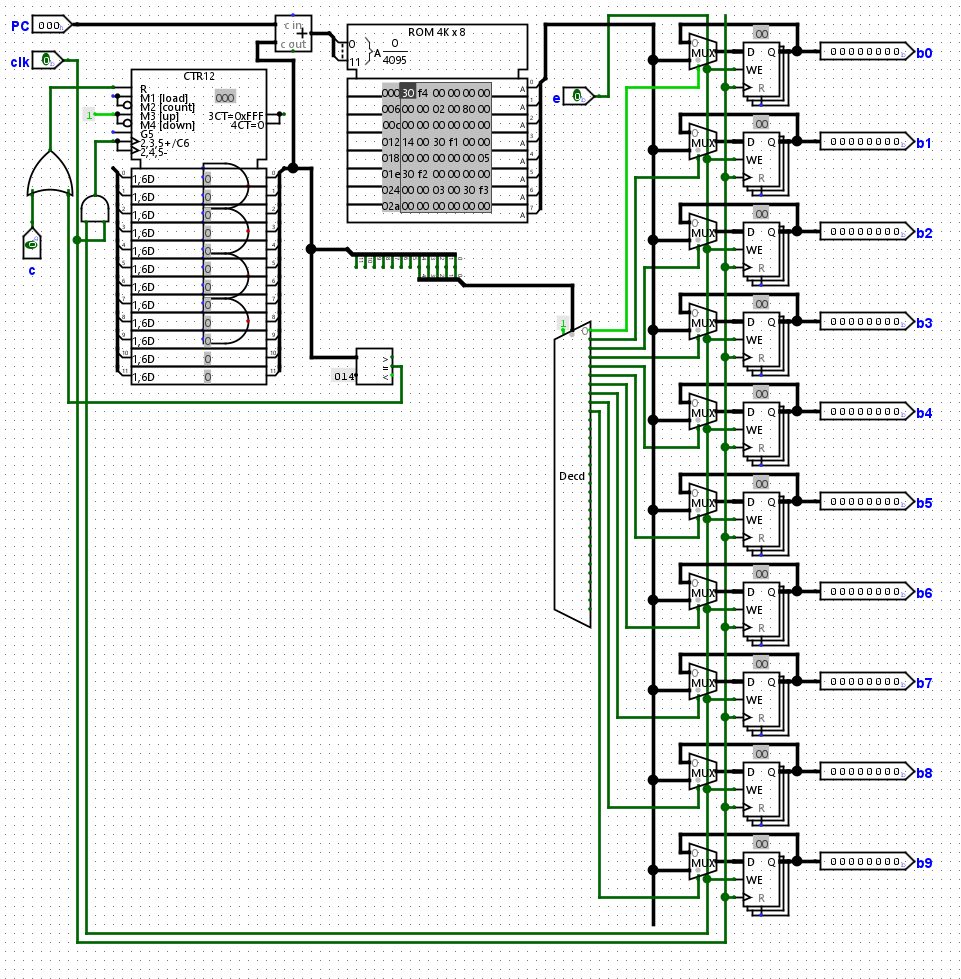
\includegraphics[scale=.45, angle=90]{instrucMem.png}
\end{center}
\subsection{Align}
The align module determines the values of \verb+rA+, \verb+rB+, and \verb+valC+ based on whether our instruction needs registers or not. When the instruction doesn't need registers we simply construct  \verb+valC+ based on the first byte being the most significant to the eighth being the least. We just let our registers still be the first byte in this case as it does not matter what is in them. When we do have registers used in our instructions we start with our most significant byte in \verb+valC+ being the second byte to the least significant being the ninth.
\begin{center}
    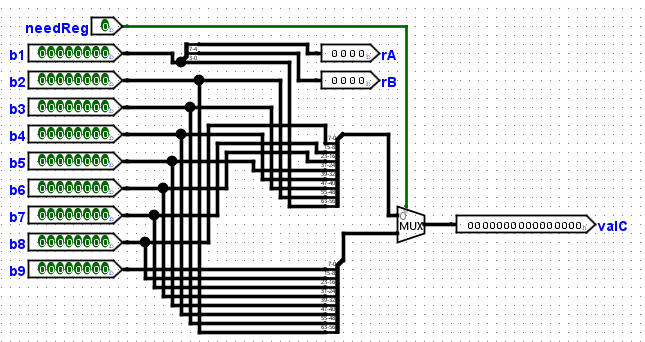
\includegraphics[scale=.7]{align.png}
\end{center}
\subsection{PC Increment}
PC increment simply increments the \verb+PC+ based on if our instruction read in registers and/or a \verb+valC+. If we read in registers we add $1$ to our \verb+PC+ and if we read in a \verb+valC+ we add $8$ to our \verb+PC+. We then also just add $1$ for our first byte containing  \verb+icode:ifun+.
\begin{center}
    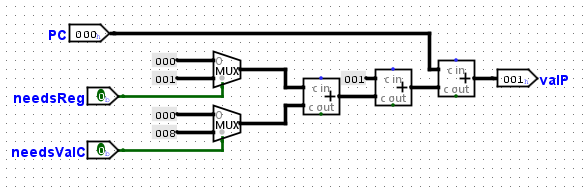
\includegraphics[scale=.5]{pcInc.png}
\end{center}
\subsection{Needs ValC and Registers}
We simply encode which instructions need a \verb+valC+ and registers based on their \verb+icode+. 
\begin{center}
    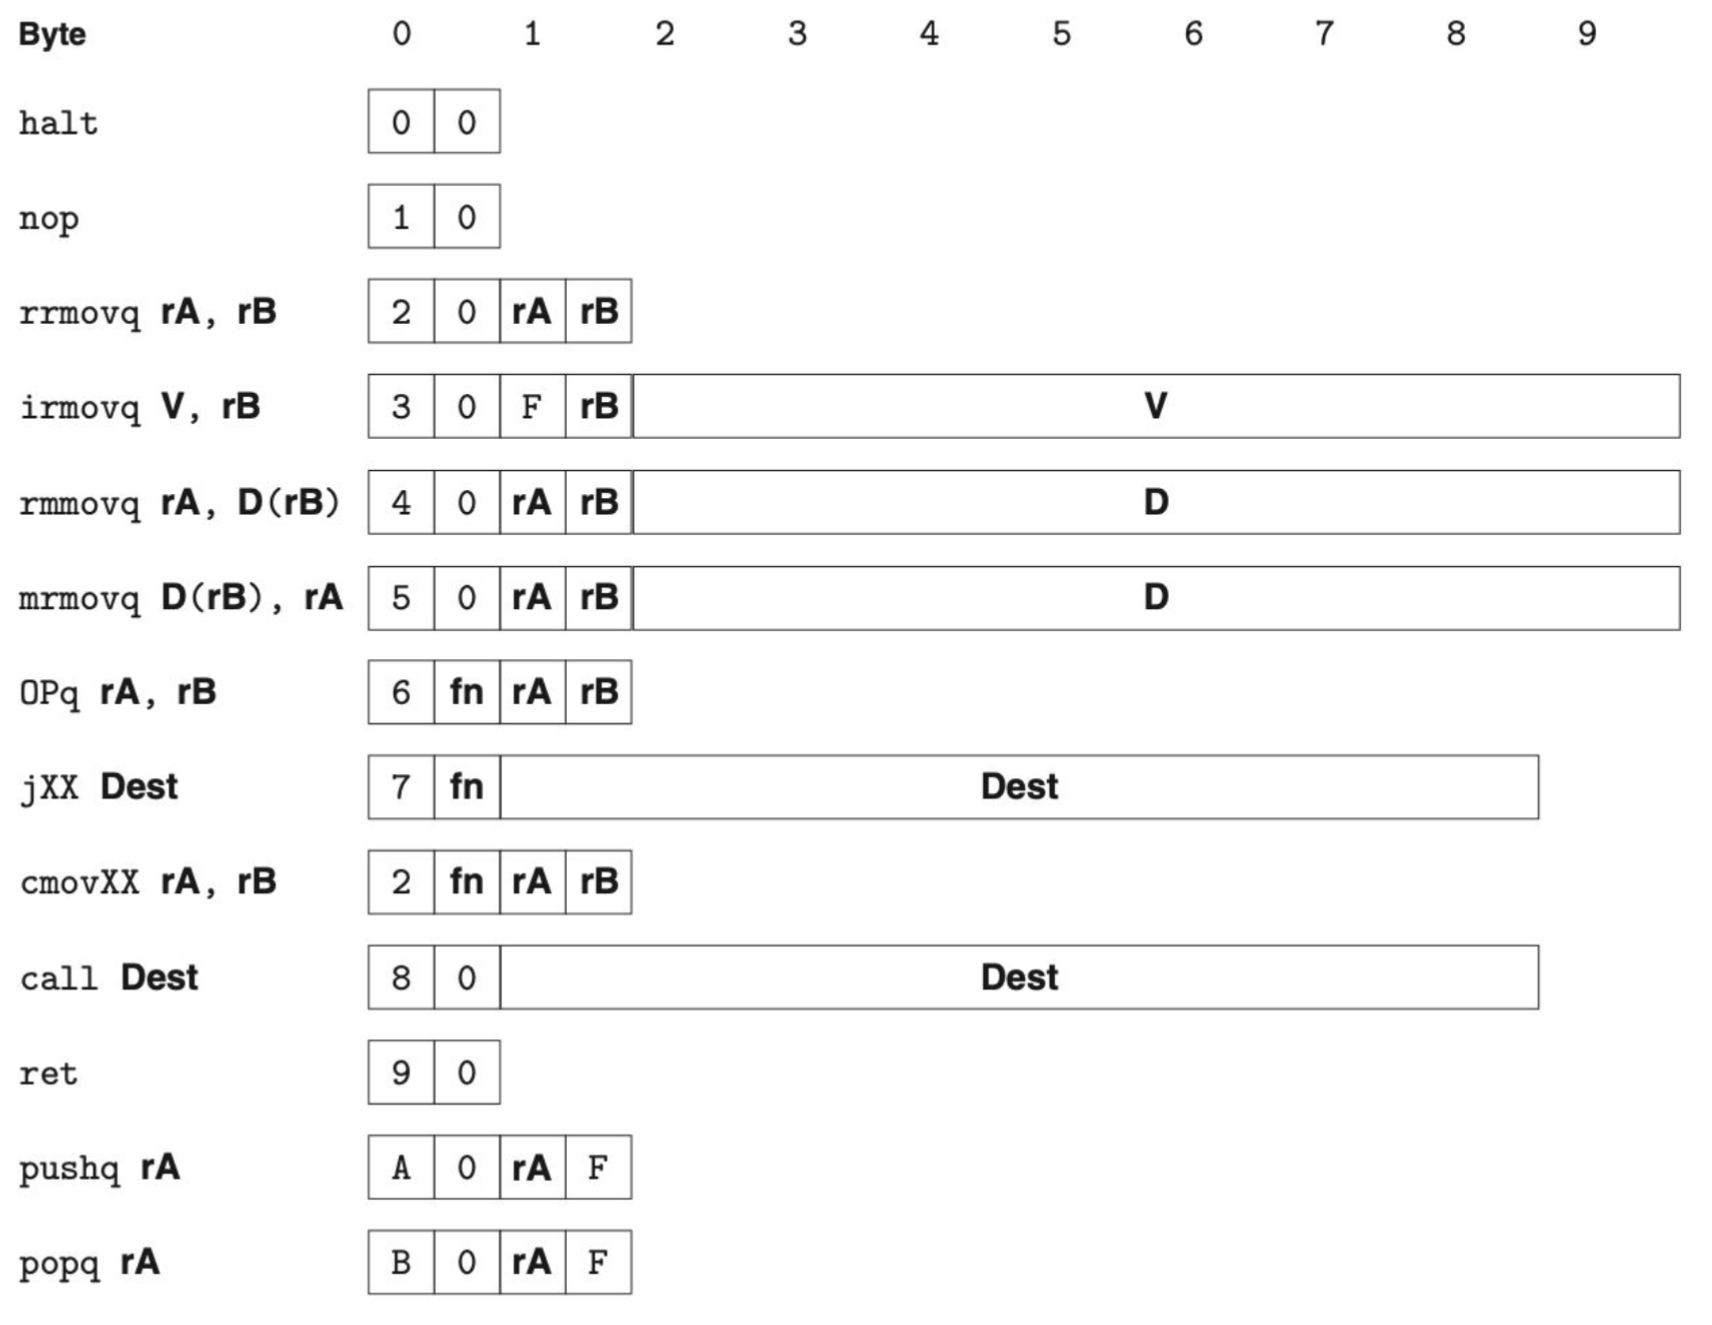
\includegraphics[scale=.6]{icode.png} \\
    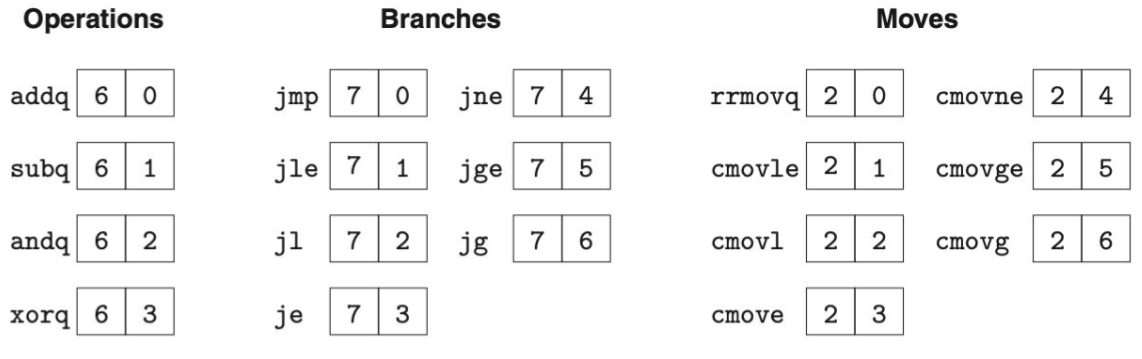
\includegraphics[scale=.8]{ops.png} 
    \\
    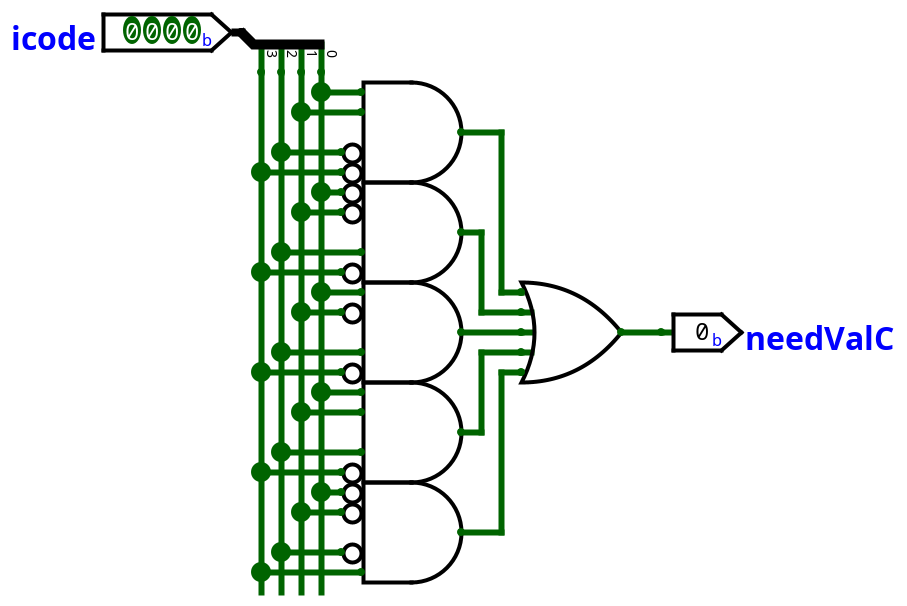
\includegraphics[scale=.7]{needsValC.png}
    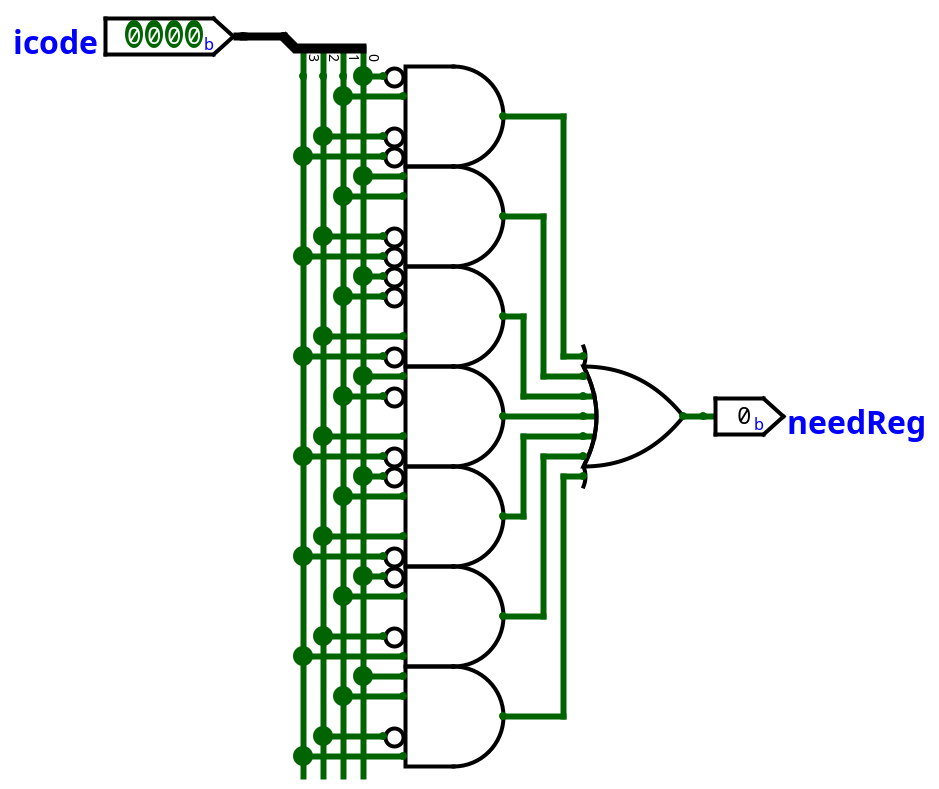
\includegraphics[scale=.7]{needsReg.png}
\end{center}
\section{Decode and Write Back Implementation}
Decode takes in 2 register addresses, rA and rB, and 2 write back values. During the decode stage, iCode to determines which registers to read from and outputs those values to valA and valB. During the write-back stage, the data is from valM and valE are written to the addresses outputted by dstM, and dstE, respectively. 
\begin{center}
    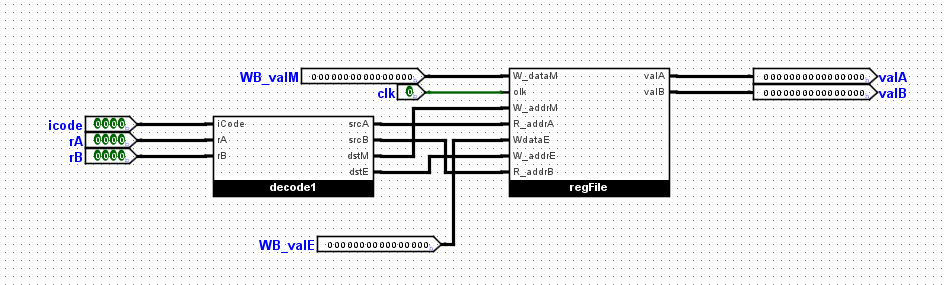
\includegraphics[scale=.6]{decode.png} \\
\end{center}
\subsection{Decode1}
Decode1 is a circuit that was built to be used to determine the values of srcA, srcB, dstM, and dstE, using iCode, rA, and rB. SrcA and srcB are 4-bit address values that tell which register addresses to read from. A multiplexer was used for each output, using iCode as the selector bit to decide which value is outputted for each value. Using the transformation table in section 1, each multiplexer was routed for each instance of iCode. When a value should not be outputted for a specific register address, 0xf is used to say there is no register to write to. For example, if srcA was 1001, the 10th register in the register file will be read from and outputted at valA.
\begin{center}
    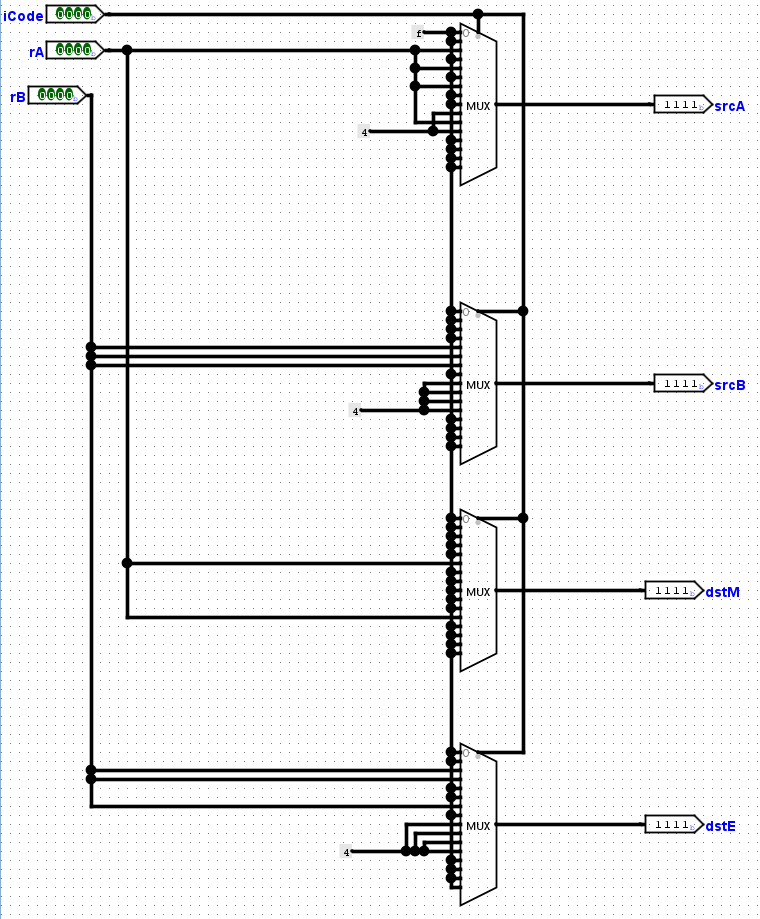
\includegraphics[scale=.6]{decode1.png} \\
\end{center}
\subsection{Register File}
RegFile is the register file used to store the values obtained during the writeback process. There are 16 registers that each hold 64-bit values, that can be accessed using 4-bit addresses. SrcA and srcB are 4-bit addresses that read the corresponding register value and output them to valA and valB respectively. When a valM or valE is supplied for dstM or dstE, those values are written to their register values to be used later on. 
\begin{center}
    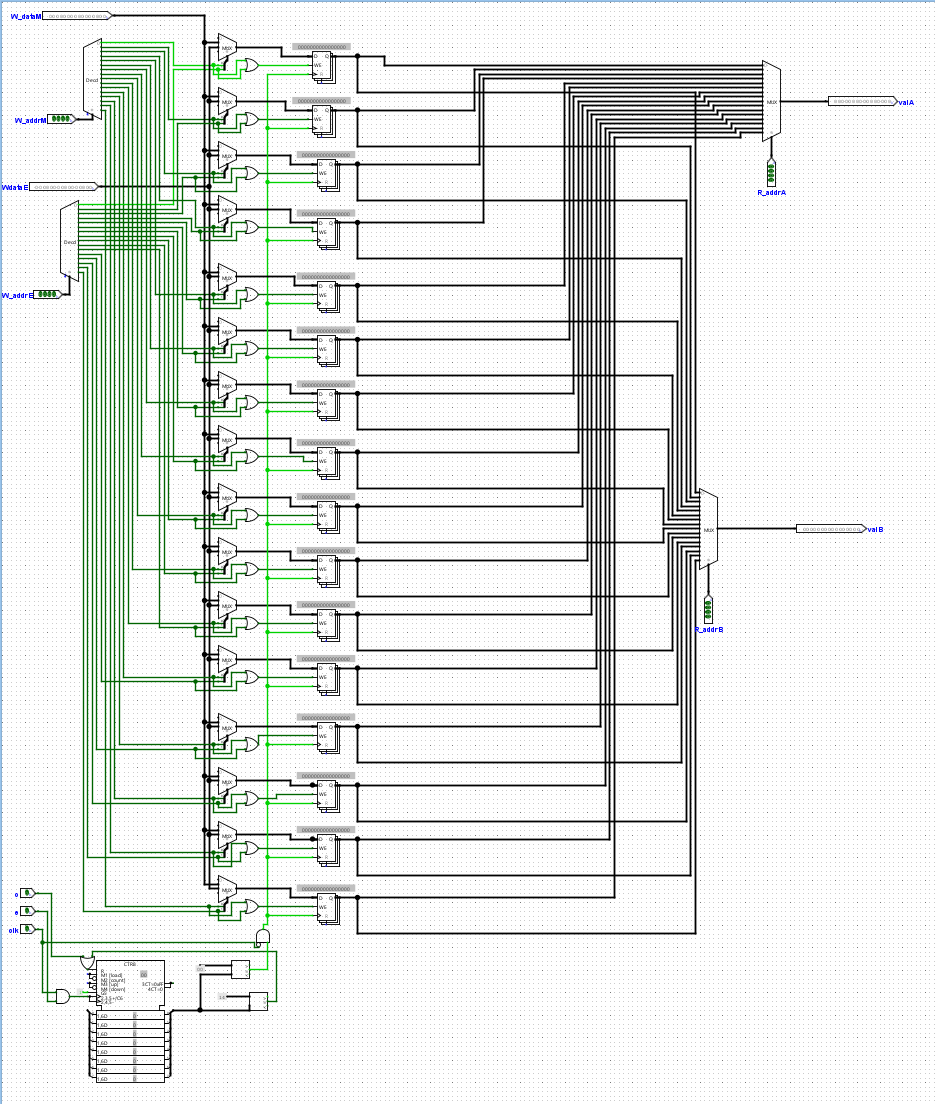
\includegraphics[scale=.6]{regFile.png} \\
\end{center}
\pagebreak
\section{Execute Implementation}
Execute uses 6 input values to perform arithmetic and logical operations on the valA, valB, or valC, given the iCode and iFun values. ICode and iFun determine which values go into which ALU circuit to then be inputted into the final ALU circuit to receive the output of valE and Cnd. 
\begin{center}
    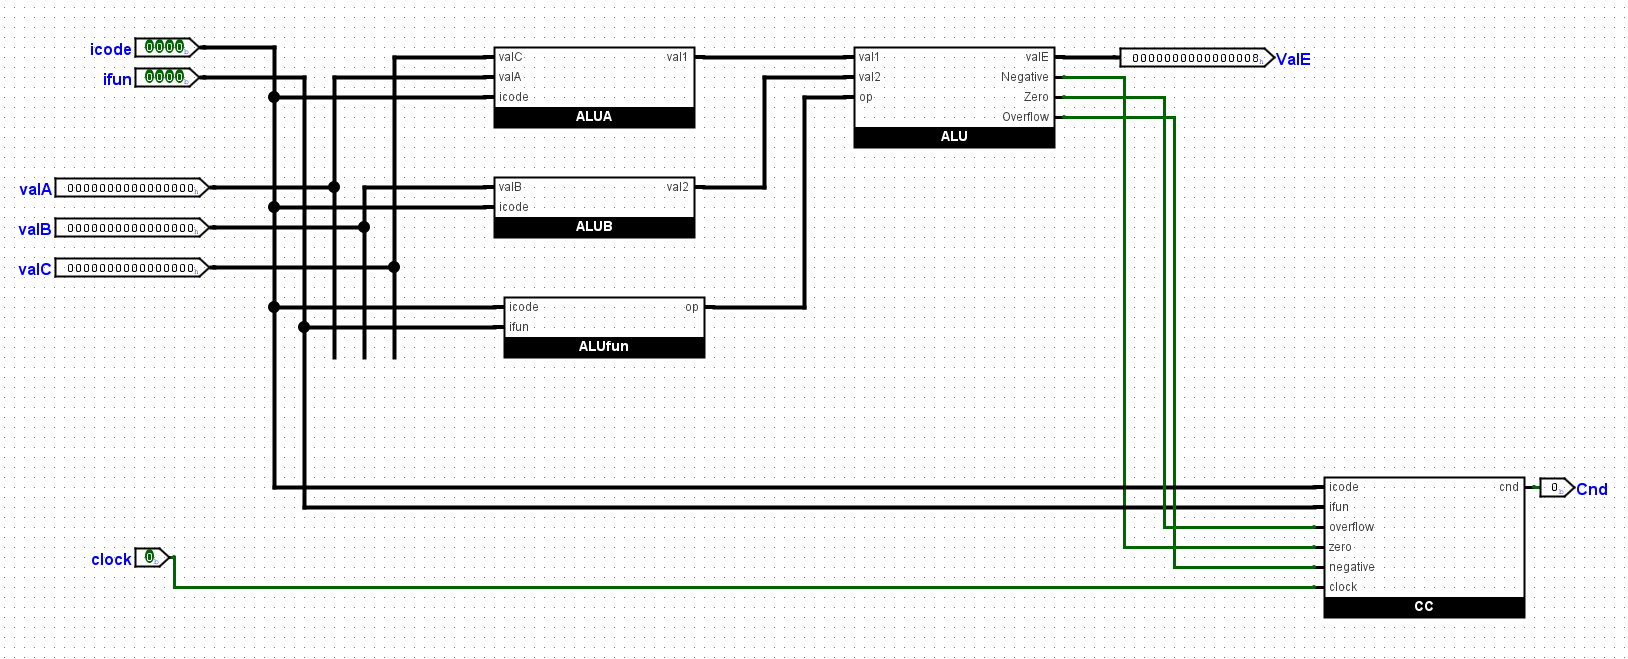
\includegraphics[scale=.4]{execute.png} \\
\end{center}
\subsection{ALU A}
ALUA takes input values of iCode, valA, and valC. When iCode is provided, it determines which values will be outputted to val1. For example, when iCode is 3, valC is outputted to val1. 
\begin{center}
    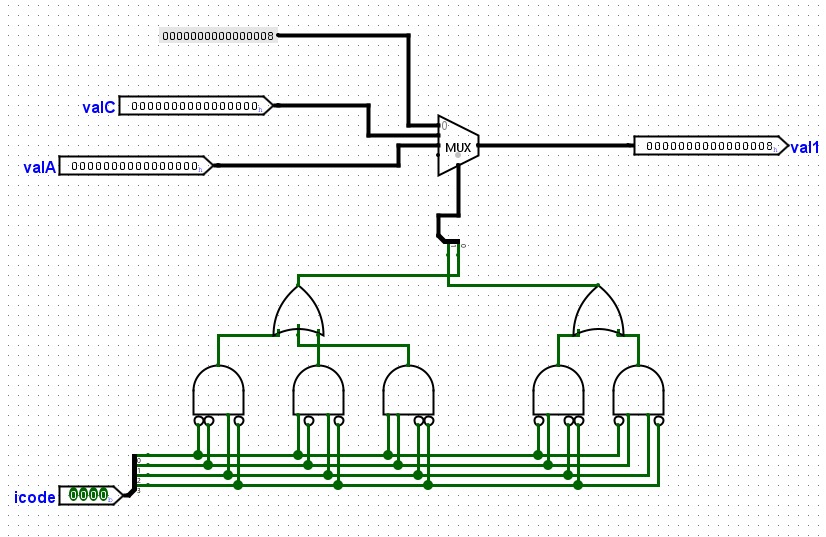
\includegraphics[scale=.6]{alu_a.png} \\
\end{center}
\pagebreak

\subsection{ALU B}
ALUB performs the same way as ALUA, but iCode determines whether 0 or valB is outputted to val2. For instance, if iCode is 4, val2 receives valB's current value. 
\begin{center}
    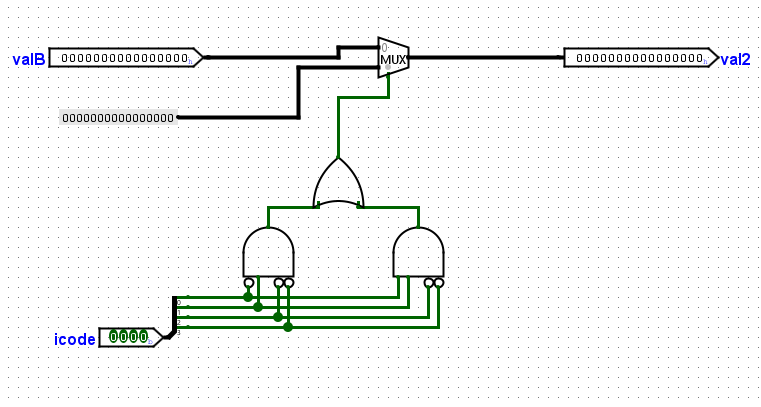
\includegraphics[scale=.7]{alu_b.png} \\
\end{center}
\subsection{ALU Function}
ALUfun takes in the values of iCode and iFun and provides a 2-bit output to tell the ALU which operation to perform. When iCode is 6 and iFun is 0, an addition operation is performed. When iCode is 6 and iFun is 1, a subtraction operation is performed, so on and so forth for each value of iCode and iFun. 
\begin{center}
    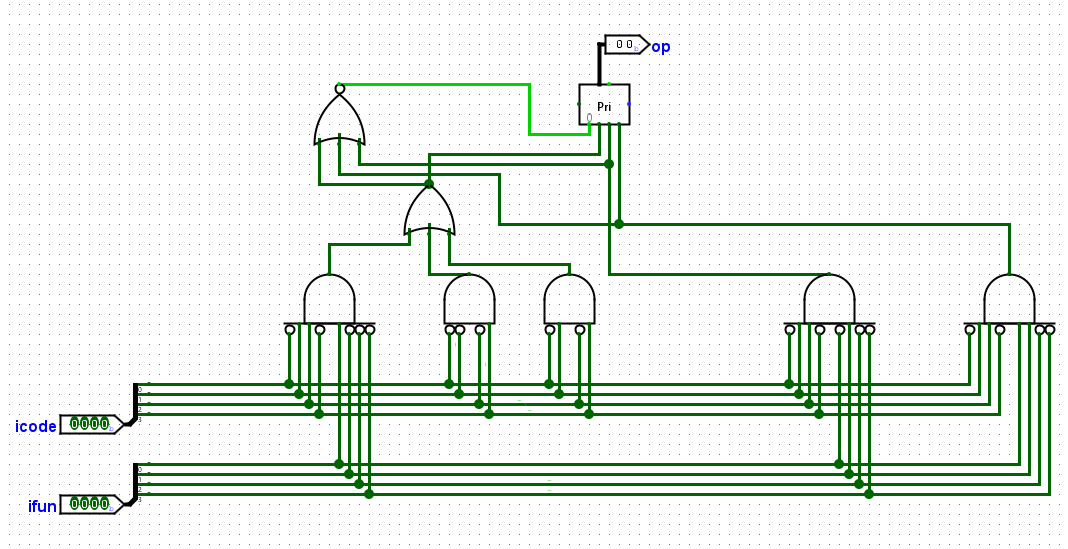
\includegraphics[scale=.6]{alu_fun.png} \\
\end{center}
\subsection{Arithmetic Logic Unit}
The ALU circuit combines all values found using iCode and iFun, and outputs the value after the operation is completed. ALU will perform all calculations no matter what value of iCode and iFun is taken in, but will only output the needed value for each required operation. This means that when "addq rA, rB" is called, it performs addition, subtraction, multiplication, and XOR, but will only output the addition value. 
\begin{center}
    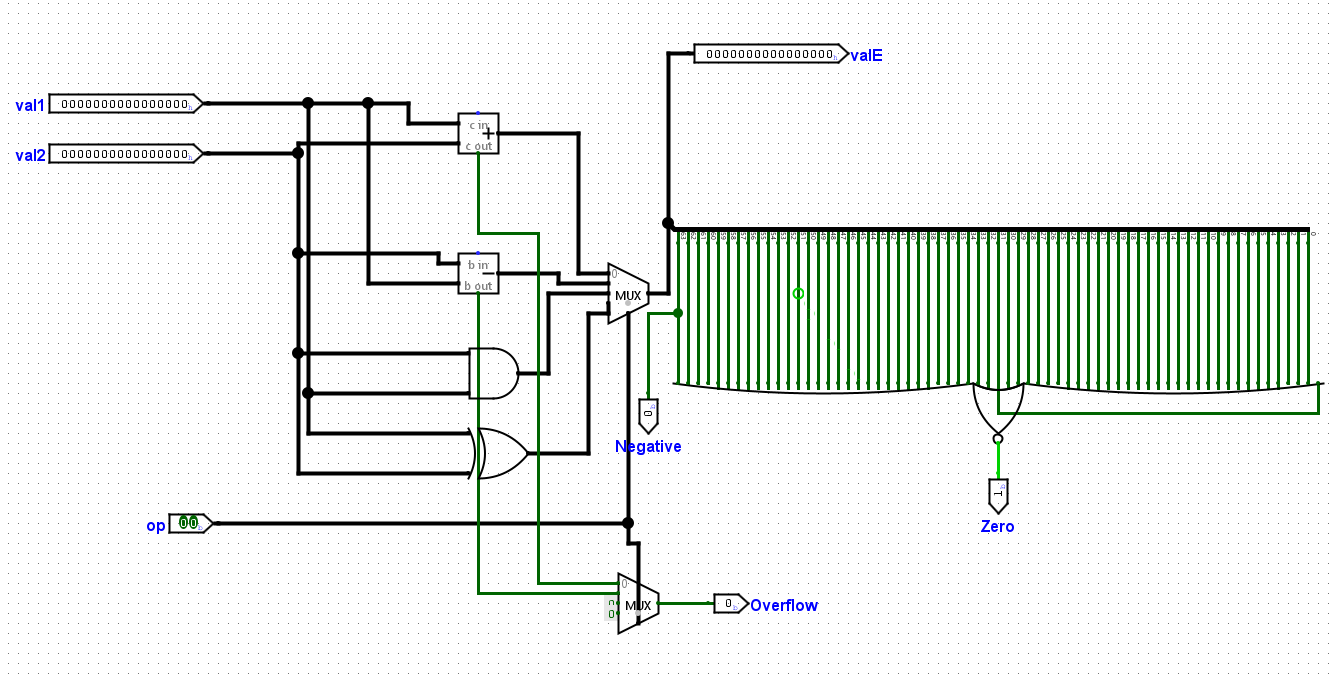
\includegraphics[scale=.5]{alu.png} \\
\end{center}
\pagebreak
\subsection{CC}
Lastly, CC determines if a flag is computed, which can be a Zero Flag, Sign Flag, and Overflow Flag. A zero flag occurs when the most recent operation yields a 0, a sign flag occurs when the most recent operation yields a negative value, and an overflow flag occurs when the most recent operation causes a two's complement overflow. This happens when ALU A and ALU B both output a value less than zero and the output computed is more than zero. CC is used to determine which jumps happen, say for instance, a "jle" line is written, if the zero flag outputs a 0, then the jump will occur. 
\begin{center}
    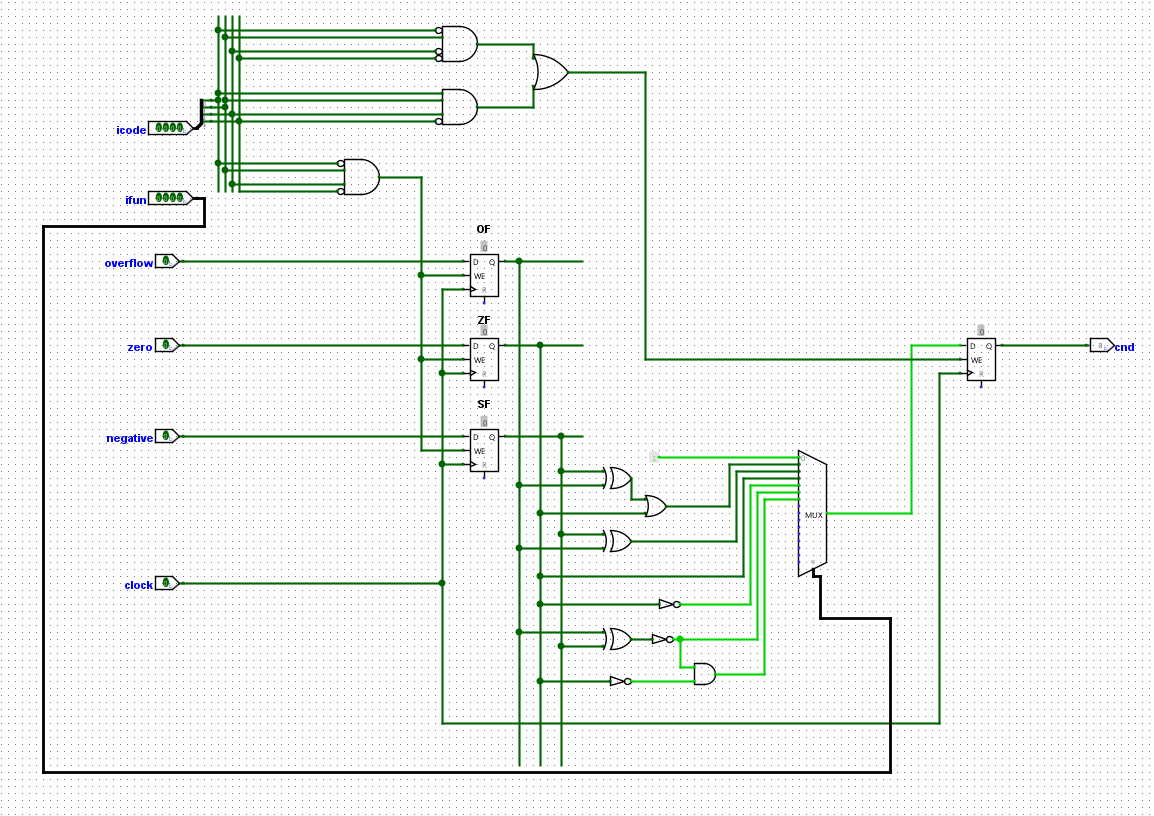
\includegraphics[scale=.5]{alu_cc.png} \\
\end{center}
\pagebreak

\section{Memory Implementation}
The memory accesses values inside the RAM and writes the data to registers to be used for processes. You also can move data from registers to memory to be used later on. The counter is used to enable the registers to read and write data during specific clock cycles 
\begin{center}
    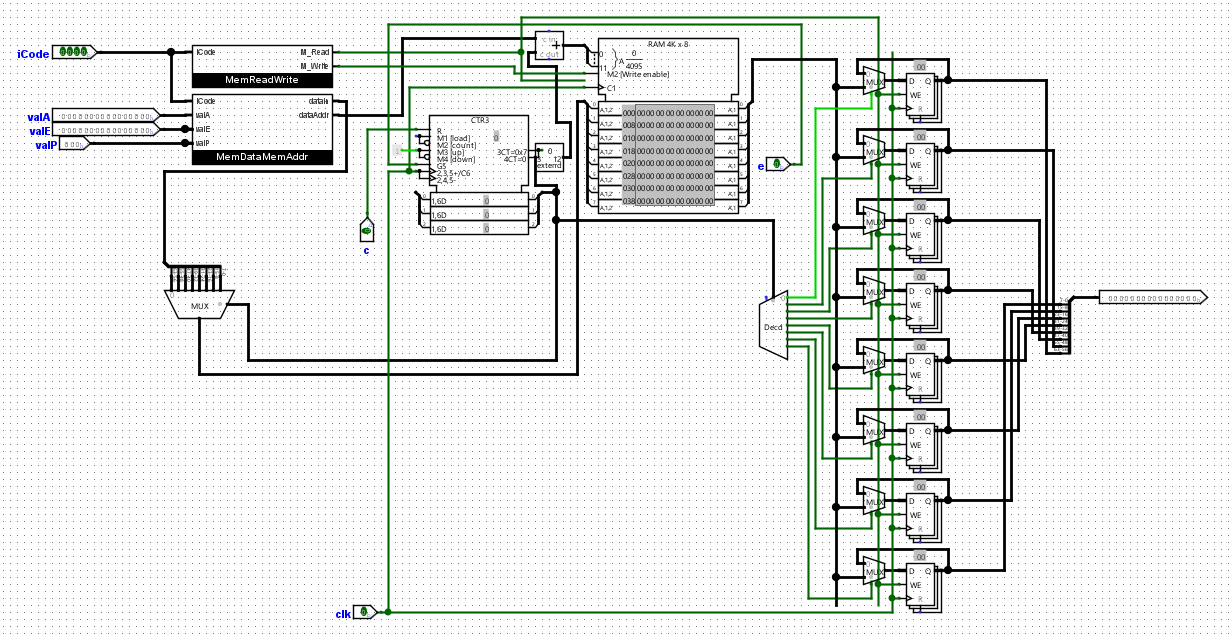
\includegraphics[scale=.5]{mem.png} \\
\end{center}
\subsection{Memory Read/Write}
The memory read and write circuit takes in the iCode value and determines if we are reading data from memory or writing data from memory. The circuit uses AND and OR gates to decide whether or not to read or write data. 
\begin{center}
    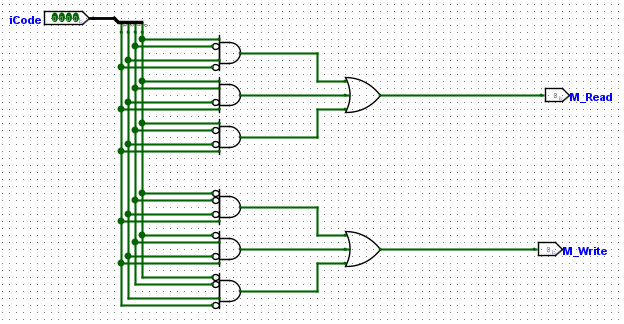
\includegraphics[scale=.8]{memreadwrite.png} \\
\end{center}
\pagebreak
\subsection{Memory Data and Memory Address}
The memory data and memory address circuit uses iCode, valA, valE, and valP to find the data and the address where we will write the data. ICode is used as a selector bit for both multiplexers, and the data address is found by taking the first 12 bits of the output for the memory address.
\begin{center}
    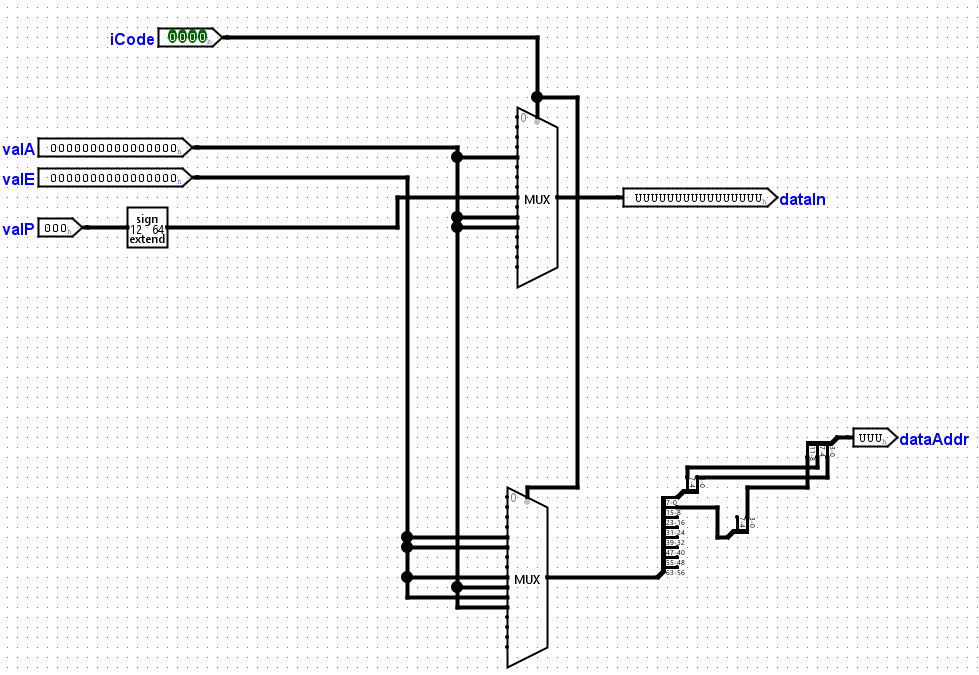
\includegraphics[scale=.6]{memaddrdata.png} \\
\end{center}

\end{document}
